\section{Teilaufgabe 1}
\begin{aufgabe}
Zeichnen Sie den Wirkungsplan der obigen Differentialgleichung und 
programmieren Sie diesen Wirkungsplan im Simulink. Füren Sie ein paar 
Simulationen durch und prüfen Sie die Plausibilität der Ergebnissen. Sie 
sollten auch unterschiedliche Anfangsbedingungen für die Drehzahl testen.
\end{aufgabe}
\begin{figure}[h!]
    \centering
    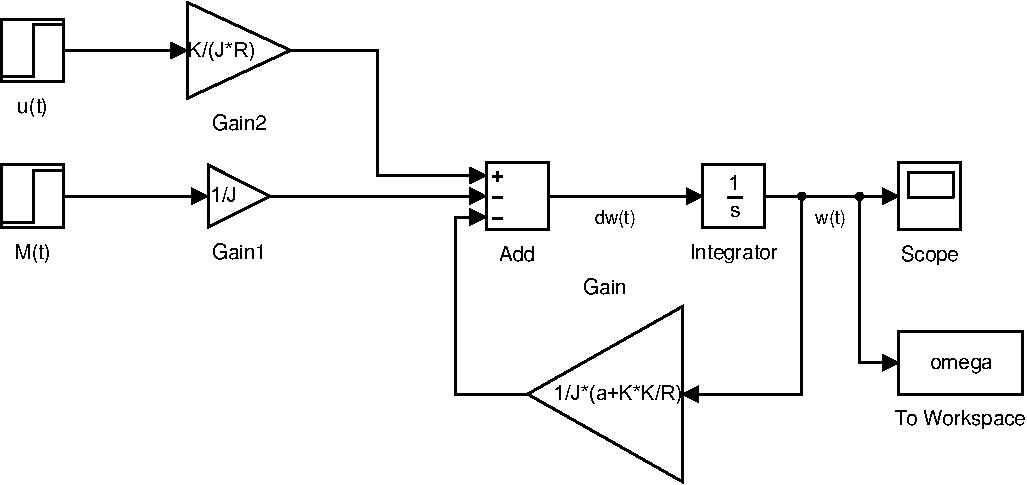
\includegraphics[width=0.6\textwidth]{01/wirkungsplan.pdf}
    \caption{Wirkungsplan DGL}
    \label{fig:01}
\end{figure}
